\begin{figure}[tb]
  \centering
  \begin{subfigure}{.49\columnwidth}
    \centering
    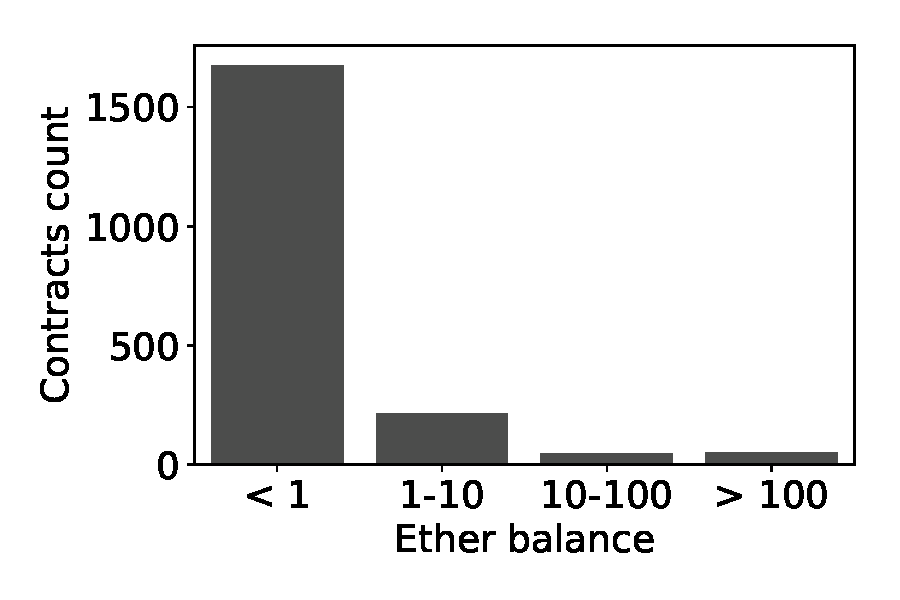
\includegraphics[width=\textwidth]{./figures/balance-histogram.pdf}
    \caption{\scriptsize Ether held by contracts in our dataset\\with non-zero balance.}
    \label{fig:eth-held}
  \end{subfigure}
  \begin{subfigure}{.49\columnwidth}
    \centering
    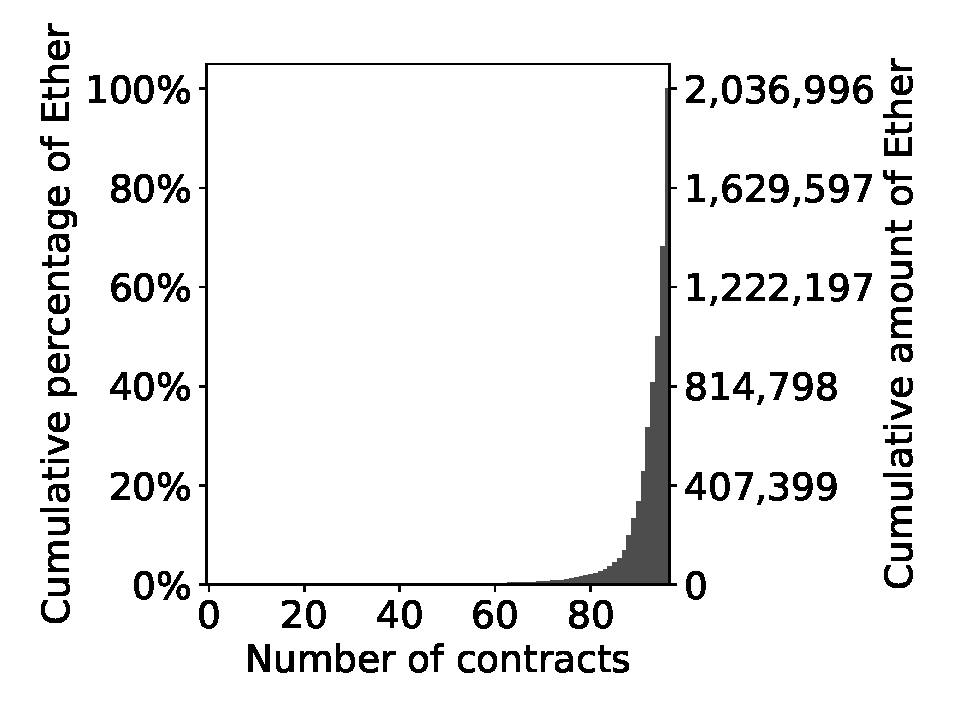
\includegraphics[width=\textwidth]{./figures/cumulative-ether.pdf}
    \caption{\scriptsize Cumulative Ether held in the 96\\contracts in our dataset containing at least 10 ETH.}
    \label{fig:cumulative-eth}
  \end{subfigure}
  \caption{Ether held in contracts: describing the distribution.}
\end{figure}

\section{Discussion}
\label{sec:discussion}

Even considering the limitations of our system, it is clear that the exploitation of smart contracts is vastly lower that what could be expected. In this section, we present some of the factors we think might be impacting the actual exploitation of smart contracts.

% \subsection{Contracts holding money}

We believe that a major reason for the difference between the number of vulnerable contracts reported and the number of contracts exploited is the distribution of Ether among contracts. Indeed, only about~\empirical{2,000} out of the~\VulnerableContracts contracts in our dataset contain Ether, and most of these contracts have a balance lower than~\empirical{1} ETH. We show the balance distribution of the contracts containing Ether in our dataset in Figure~\ref{fig:eth-held}. Furthermore, the \empirical{top 10 contracts} hold about~\empirical{95\%} of the total Ether. We show the cumulative distribution of Ether within the contracts containing more than~\empirical{10 ETH} in Figure~\ref{fig:cumulative-eth}. This shows that, as long as the top contracts cannot be exploited, the total amount of Ether that is actually at stake will be nowhere close to the upper bound of ``vulnerable'' Ether.

To make sure this fact generalizes to the whole Ethereum blockchain and not only our dataset, we fetch the balances for all existing contracts. This gives a total of~\empirical{15,459,193} contracts. Out of these, we find that only~\empirical{463,538} contracts have a non-zero balance, which is merely 3\% of all the contracts. Out of the contracts with a non-zero balance, the top 10 contracts account for \empirical{54\%} of the total amount of Ether, the top 100 for \empirical{92\%} and the top 1000 for \empirical{99\%}. This shows that our dataset follows the same trend as the Ethereum blockchain in general: a very small amount of contracts hold most of the wealth.

\point{Manual inspection of high value contracts}
We decide to manually inspect the top~\empirical{6} contracts~ ---~i.e contracts with the highest balances at the time of writing~ ---~marked as vulnerable by any of the tools in our dataset. We focused on the top~\empirical{6} because it happened to be the number of contracts which currently hold more than~\empirical{100,000 ETH}. These contracts hold a total of~\empirical{1,695,240} ETH, or~\empirical{83\%} of the total of \empirical{2,037,521 ETH} currently held by all the contracts in our dataset. We give an overview of the findings here and a more in-depth version in Appendix~\ref{sec:investigations}.

\begin{figure*}[tb]
  \centering
  \small
  \begin{tabular}{lrll}
    \toprule
    \bf Address & \bf Ether balance & \bf Deployment date  & \bf Flagged vulnerabilities\\
    \midrule
    \addr[\footnotesize]{0xde0b295669a9fd93d5f28d9ec85e40f4cb697bae} & 649,493 & 2015-08-08 & Oyente: \vre\\
    \midrule
    \addr[\footnotesize]{0x7da82c7ab4771ff031b66538d2fb9b0b047f6cf9} & 369,023 & 2016-11-10 & MadMax:~\vle, Zeus:~\vio\\
    \midrule
    \addr[\footnotesize]{0x851b7f3ab81bd8df354f0d7640efcd7288553419} & 189,232 & 2017-04-18 & MadMax:~\vle\\
    \midrule
    \addr[\footnotesize]{0x07ee55aa48bb72dcc6e9d78256648910de513eca} & 182,524 & 2016-08-08 & Securify:~\vre\\
    \midrule
    \addr[\footnotesize]{0xcafe1a77e84698c83ca8931f54a755176ef75f2c} & 180,300 & 2017-06-04 & MadMax:~\vle\\
    \midrule
    \addr[\footnotesize]{0xbf4ed7b27f1d666546e30d74d50d173d20bca754} & 124,668 & 2016-07-16 & Securify:~\vto,~\vue; Zeus:~\vle,~\vio\\
    \bottomrule
  \end{tabular}
  \caption{Top \empirical{six} most valuable contracts flagged as vulnerable by at least one tool.}
  \label{fig:vulnerable-active}
\end{figure*}

\begin{investigation}{0xde0b295669a9fd93d5f28d9ec85e40f4cb697bae}
The source code for this contract is not available on Etherscan. However, we discovered that this is the multi-signature wallet of the Ethereum foundation~\cite{ether-foundation-contract-reddit} and that its source code is available on GitHub~\cite{ether-foundation-contract-code}. We inspect the code and find that the only calls taking place require the sender of the message to be an owner. This by itself is enough to prevent any re-entrant call, as the malicious contract would have to be an owner, which does not make sense. Furthermore, although the version of Oyente used in the paper reported the re-entrancy, more recent versions of the tool did not report this vulnerability anymore. Therefore, we safely conclude that the re-entrancy issue was a false alert.
\end{investigation}

We were able to inspect~\empirical{4} of the~\empirical{5} remaining contracts. The contract at address~\addr[\footnotesize]{0x07ee55aa48bb72dcc6e9d78256648910de513eca} is the only one for which we were unable to find any information. The second, third and fifth contracts in the list were also multi-signature wallets and exploitation would require a majority owner to be malicious. For example, for Ether to get locked, the owners would have to agree on adding enough extra owners so that all the loops over the owners result in an out-of-gas exception. The contract at address~\addr[\footnotesize]{0xbf4ed7b27f1d666546e30d74d50d173d20bca754} is a contract known as \lstinline{WithDrawDAO}~\cite{withdraw-dao}. We did not find any particular issue, but it does use a delegate pattern which explains the locked Ether vulnerability marked by Zeus.

We present a thorough investigation of the high-value contracts in Appendix~\ref{sec:investigations}. Overall, all the contracts from Figure~\ref{fig:vulnerable-active} that we could analyze seemed quite secure and the vulnerabilities flagged were definitely not exploitable. Although there are some very rare cases that we present in Section~\ref{sec:related} where contracts with high Ether balances are being stolen, these remain exceptions. The facts we presented up to now help us confirm that the amount of Ether at risk on the Ethereum blockchain is nowhere as close as what is claimed~\cite{DBLP:conf/ndss/KalraGDS18,Grech2018}.

% \subsection{Lifespan of contracts}
% As described in Section~\ref{sec:background}, due to smart contracts deployed on Ethereum being immutable, any update to a contract requires the deployment of a new one. As a result, smart contracts have a relatively short lifespan. We define the lifespan of a smart contract as the number of days elapsed between the first and the last transaction sent to it.

% \begin{figure}[tb]
%     % \includegraphics[width=\columnwidth]{./figures/recency.pdf}
%     \caption{Capturing the recency of active contract use.}
%     \label{fig:recency}
% \end{figure}
% Figure~\ref{fig:recency}...
